\begin{frame}
  \frametitle{MOOSE Framework}
  \begin{columns}
    \column[t]{6cm}
  \begin{figure}[t]
     \vspace{-0.25in}
       \hspace*{-0.25in}
       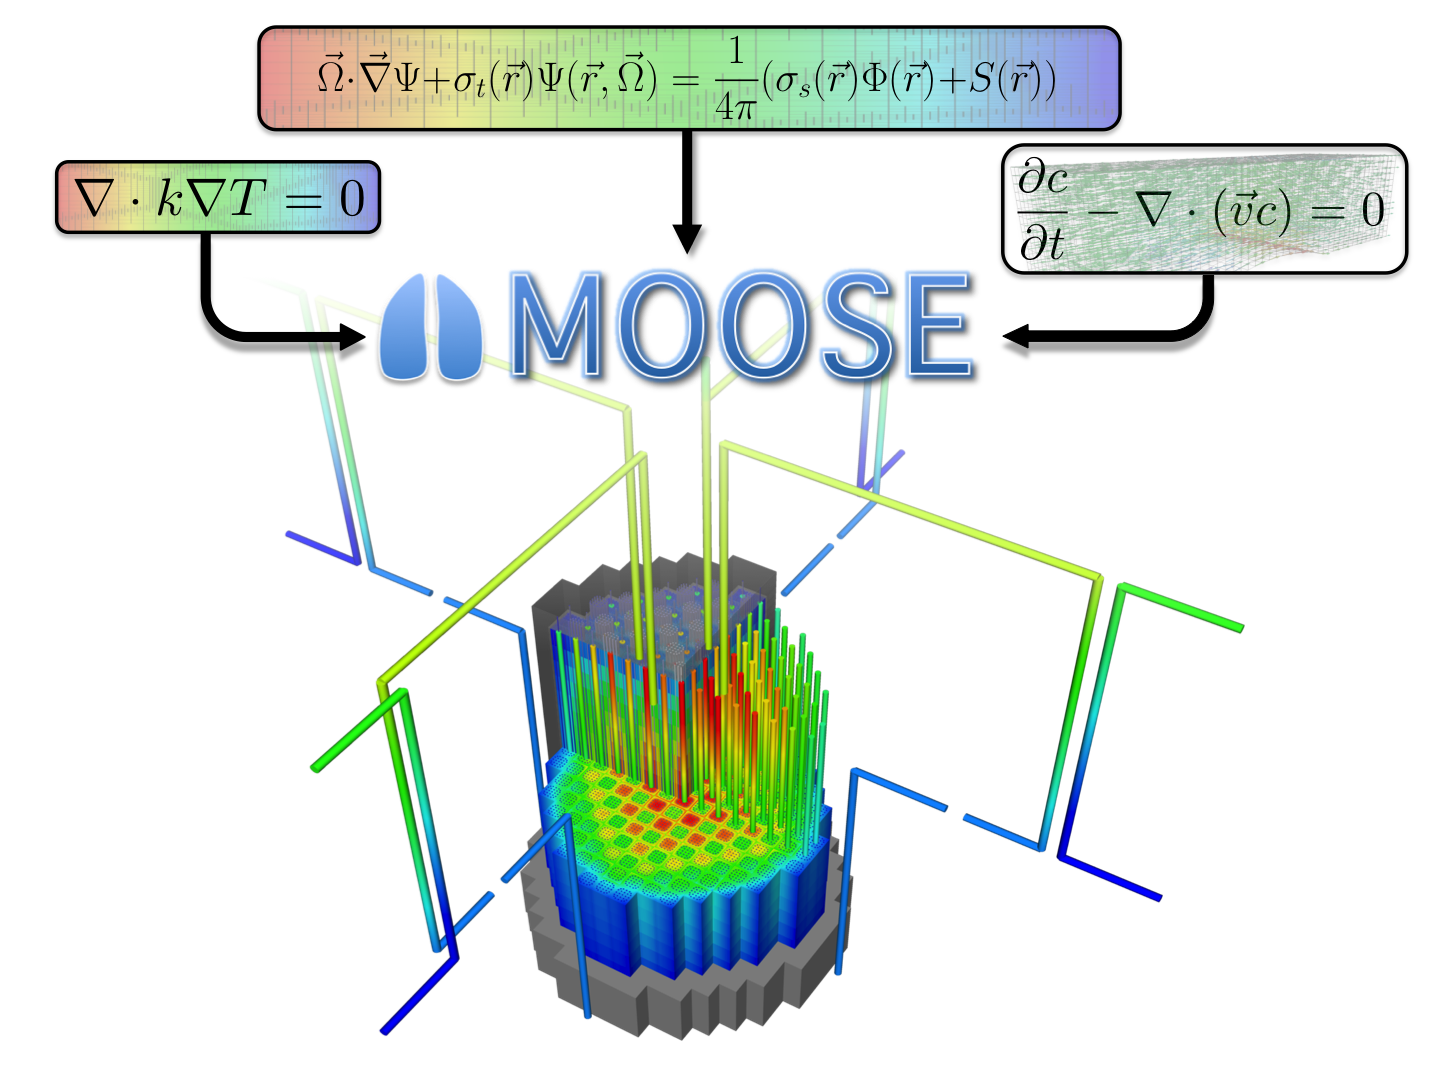
\includegraphics[height=0.65\textheight]{./images/moose.png}
            \caption{Multi-physics Object-Oriented Simulation Environment (MOOSE).}
  \end{figure}
	\column[t]{6cm}
               \begin{itemize}
	       \item Fully-coupled, fully-implicit multiphysics solver
               \item MOOSE interfaces with libMesh to discretize simulation volume into finite elements
               \item Residuals and Jacobians handed off to PetSc which handles solution of resulting non-linear system of algebraic equations
	       \item Automatically parallel (largest runs \textgreater 100,000 CPU cores!)
	       \item Built-in mesh adaptivity
	       \item Intuitive parallel multiscale solves
               \end{itemize}

  \end{columns}
\end{frame}

\begin{frame}
        \frametitle{Moltres (Coupling in MOOSE)}
  \begin{figure}
   \vspace{-0.05in}
   \hspace*{-0.15in}
   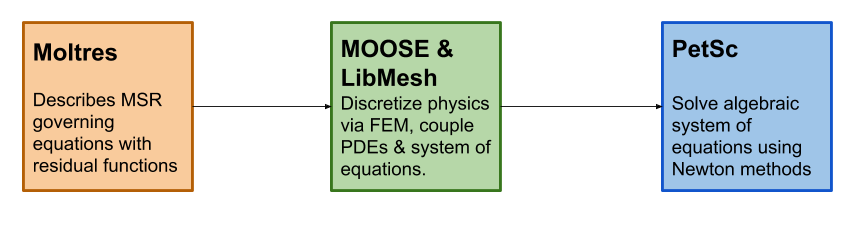
\includegraphics[width=1.1\textwidth]{./images/moltres-moose-diag.png}
    \end{figure}
\end{frame}

\begin{frame}
        \frametitle{Inro to Moltres}
        \begin{itemize}  
                \item Fluid-fuelled, molten salt reactors
                \item Multi-group diffusion (arbitrary groups)
                \item Advective movement of delayed neutron precursors
                \item Navier-Stokes thermal hydraulics
                \item 3D unstructured
                \item 2D axisymmetric
                \item 3D structured 
                \item Initial developer: Alexander Lindsay
        \end{itemize}
\end{frame}

\begin{frame}
        \frametitle{Acquiring Moltres}
             \texttt{git clone https://github.com/arfc/moltres}\\
        \texttt{cd moltres}\\
        \texttt{git submodule init}\\
        \texttt{git submodule update}\\
\end{frame}

\begin{frame}
        \frametitle{Diffusion in Moltres}
        \footnotesize{
        \begin{align}
        \frac{1}{v_g}\frac{\partial \phi_g}{\partial t} &- \nabla \cdot D_g
        \nabla \phi_g + \Sigma_g^r \phi_g =\\
                &\sum_{g \ne g'}^G \Sigma_{g'\rightarrow g}^s \phi_{g'} + \chi_g^p \sum_{g' = 1}^G (1 -
        \beta) \nu \Sigma_{g'}^f \phi_{g'} + \chi_g^d \sum_i^I \lambda_i C_i
        \end{align}}
\begin{columns}
    \begin{column}{0.48\textwidth}
        \footnotesize{
        \begin{align*}
                v_g &= \mbox{speed of neutrons in group g} \\
                \phi_g &= \mbox{flux of neutrons in group g} \\
                t &= \mbox{time} \\
                D_g &= \mbox{Diffusion coefficient for neutrons in group g} \\
                \Sigma_g^r &= \mbox{macroscopic cross-section for}\\
                &\mbox{removal of neutrons from group g} \\
                \Sigma_{g'\rightarrow g}^s &= \mbox{macroscopic cross-section 
                of}\\
                &\mbox{  scattering from g' to g} \\
                \chi_g^p &= \mbox{prompt fission spectrum, neutrons in group g} \\
        \end{align*}}
    \end{column}
    \begin{column}{0.48\textwidth}
        %Content
        \footnotesize{
        \begin{align*}
                G &= \mbox{number of discrete groups, g} \\
                \nu &= \mbox{neutrons produced per fission} \\
                \Sigma_g^f &= \mbox{macroscopic fission cross section}\\
                &\mbox{ due to neutrons in group g} \\
                \chi_g^d &= \mbox{delayed neutrons in group g} \\
                I &= \mbox{ delayed neutron precursor groups} \\
                \beta &= \mbox{delayed neutron fraction}\\
                \lambda_i &= \mbox{average decay constant}\\
                &\mbox{of delayed neutron precursors in group i} \\
                C_i &= \mbox{concentration of delayed neutron}\\
                &\mbox{precursors in precursor group i}\\.
        \end{align*}}
    \end{column}
\end{columns}
\end{frame}

\begin{frame}
        \frametitle{Moltres Delayed Neutrons}
        \begin{align}
        \frac{\partial C_i}{\partial t} &= \sum_{g'= 1}^G \beta_i \nu
        \Sigma_{g'}^f \phi_{g'} - \lambda_i C_i - \frac{\partial}{\partial z} u
        C_i \label{eq:precursors}
\end{align}

        \begin{align*}
                G &= \mbox{number of discrete groups, g} \\
                I &= \mbox{ delayed neutron precursor groups} \\
                C_i &= \mbox{concentration of delayed neutron}\\
                &\mbox{precursors in precursor group i}\\.
                u &= \mbox{vertical fluid velocity}\\
                \lambda_i &= \mbox{average decay constant}\\
                &\mbox{of delayed neutron precursors in group i} \\
                \beta &= \mbox{fraction of delayed neutron}\\
                &\mbox{precursors in group i} \\
        \end{align*}
\end{frame}


\begin{frame}
        \frametitle{Moltres Fuel Temperature}
\begin{align}
        \rho_fc_{p,f}\frac{\partial T_f}{\partial t} &+ \nabla\cdot\left(\rho_f
        c_{p,f} \vec{u}\cdot T_f -k_f\nabla T_f\right) =  Q_f
\end{align}
\begin{align}
  \rho_f &= \mbox{density of fuel salt}\\
  c_{p,f} &= \mbox{specific heat capacity of fuel salt}\\
  T_f &= \mbox{temperature of fuel salt}\\
  \vec{u} &= \mbox{velocity of fuel salt}\\
  k_f &= \mbox{thermal conductivity of fuel salt}\\
  Q_f &= \mbox{source term} = \sum_{g=1}^G \epsilon_{f,g}\Sigma_{f,g}\phi_g
\end{align}
\end{frame}


\begin{frame}
        \frametitle{Moltres Moderator Temperature}
\begin{align}
        \rho_gc_{p,g}\frac{\partial T_g}{\partial t} &+
        \nabla\cdot\left(-k_g\nabla T_g\right) =  Q_g\\
\end{align}
\begin{align}
  \rho_g &= \mbox{density of graphite moderator}\\
  c_{p,g} &= \mbox{specific heat capacity of graphite moderator}\\
  T_g &= \mbox{temperature of graphite moderator}\\
  k_g &= \mbox{thermal conductivity of graphite moderator}\\
  Q_g &= \mbox{source term in graphite moderator}\\
\end{align}

\end{frame}


\begin{frame}
        \frametitle{Moltres MSRE Simulation}
  \begin{figure}
   \vspace{-0.05in}
   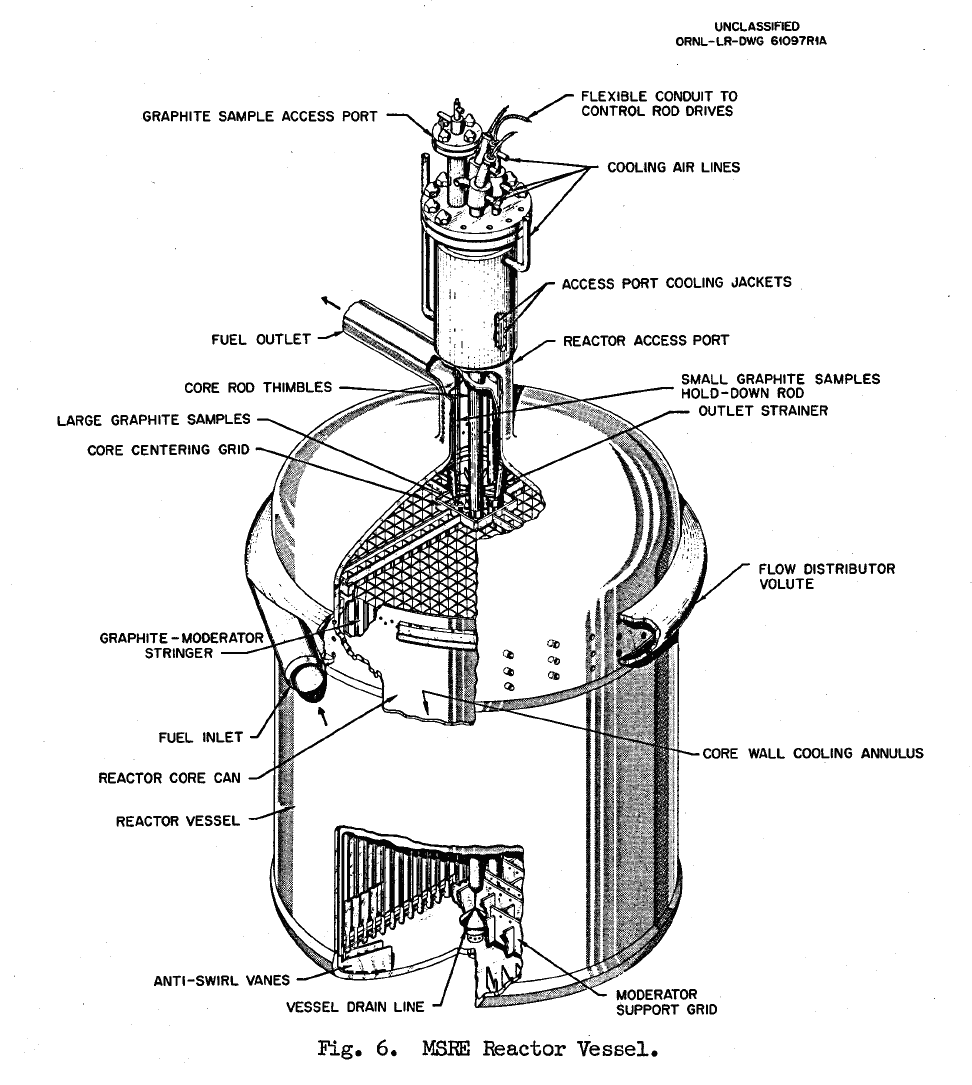
\includegraphics[height=0.85\textheight]{./images/msre.png}
    \end{figure}
\end{frame}


\begin{frame}
        \frametitle{Moltres MSRE Simulation}
  \begin{figure}
   \vspace{-0.05in}
   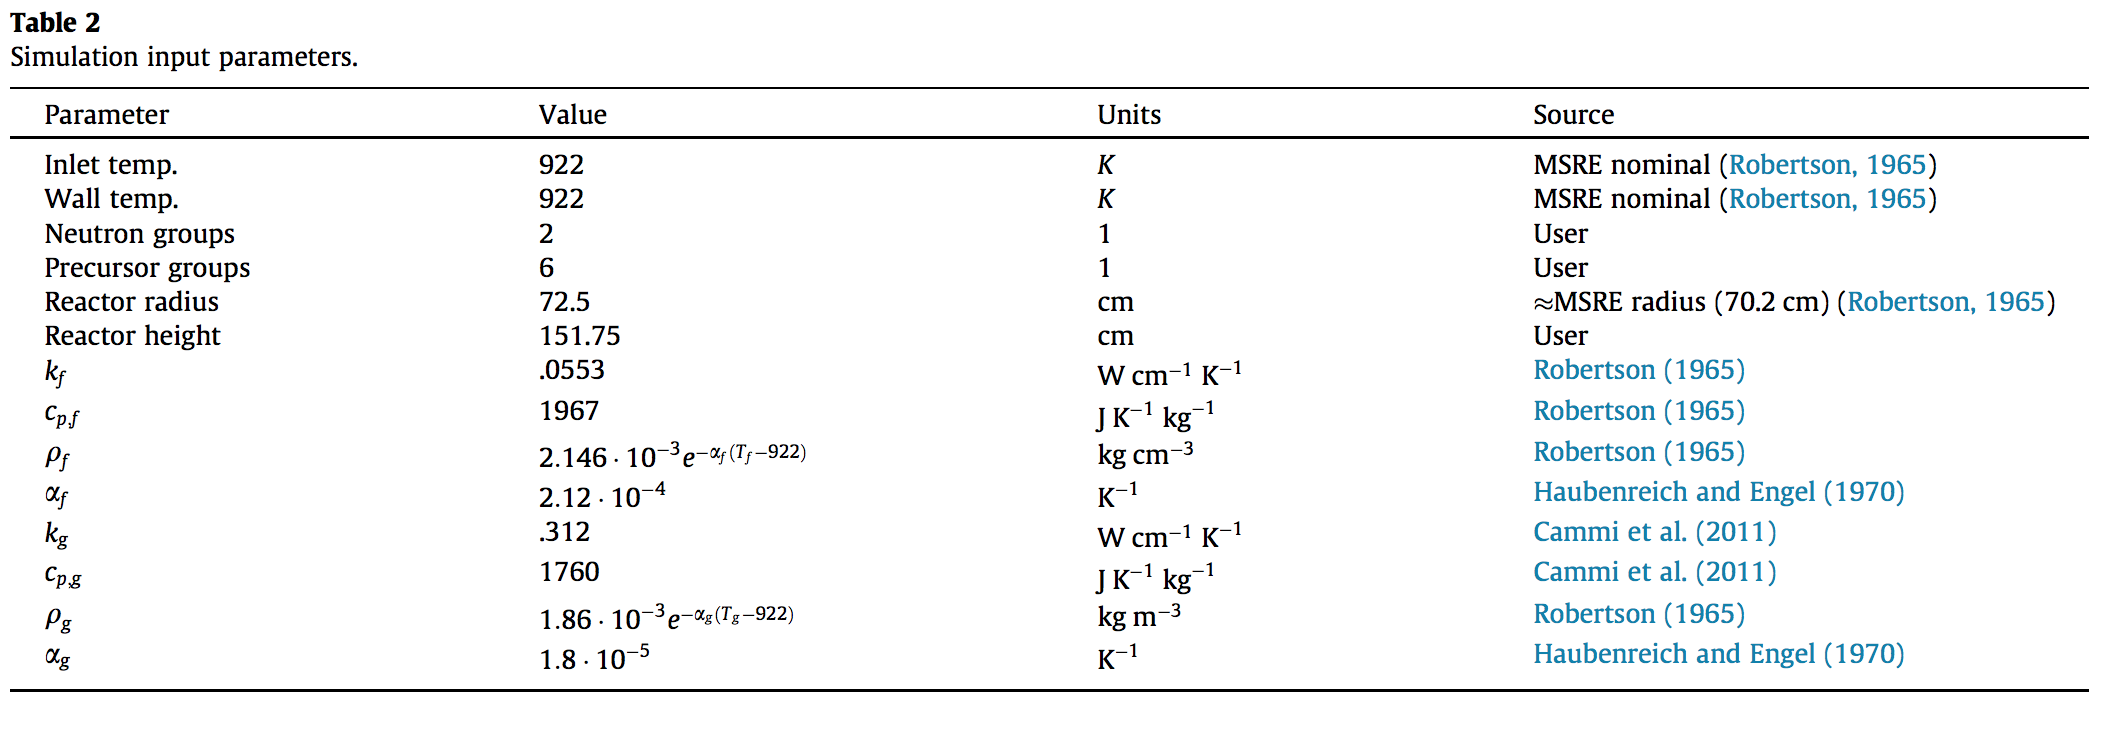
\includegraphics[width=1.2\textwidth]{./images/moltres-input.png}
          \caption{Data used in \cite{lindsay_introduction_2018}.}
    \end{figure}
\end{frame}

\begin{frame}
        \frametitle{Moltres MSRE Simulation}
  \begin{figure}
   \vspace{-0.05in}
   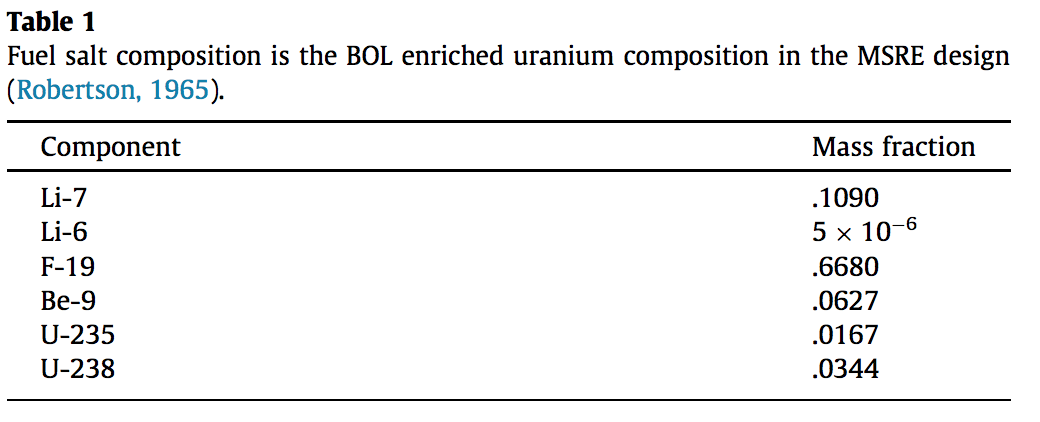
\includegraphics[width=0.85\textwidth]{./images/moltres-composition.png}
          \caption{Data used in \cite{lindsay_introduction_2018}.}
    \end{figure}
\end{frame}


\begin{frame}
        \frametitle{Moltres (coupling in MOOSE)}
  \begin{figure}
   \vspace{-0.05in}
   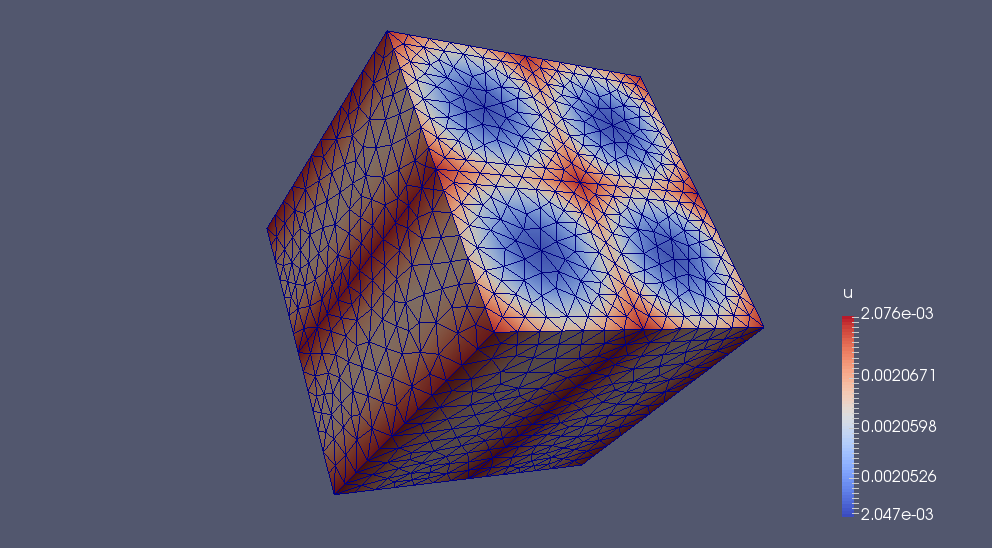
\includegraphics[height=0.85\textheight]{./images/lindsay_msre_moose.png}
    \end{figure}
\end{frame}



\begin{frame}
        \frametitle{Moltres Precursor Drift}
  \begin{figure}
   \vspace{-0.1in}
   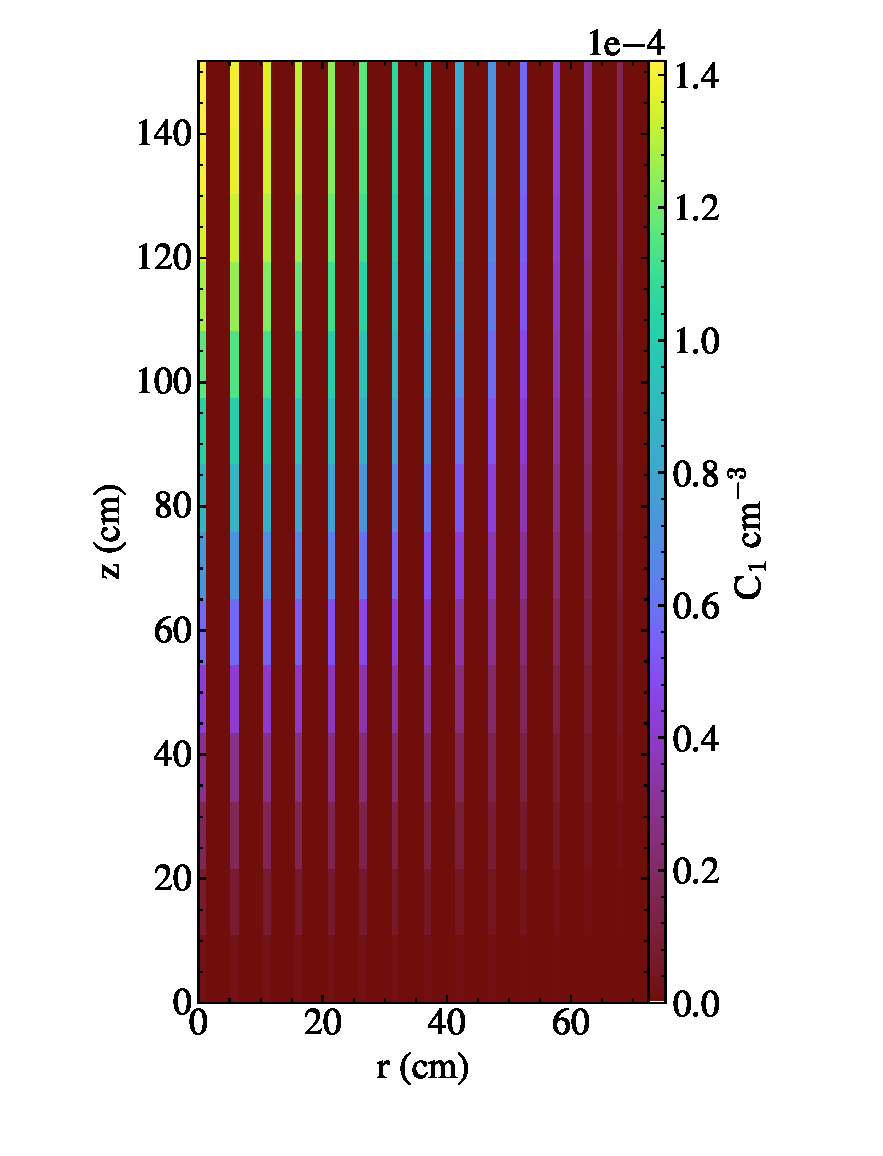
\includegraphics[width=0.28\textwidth]{./images/auto_diff_rho_pre1.eps}
   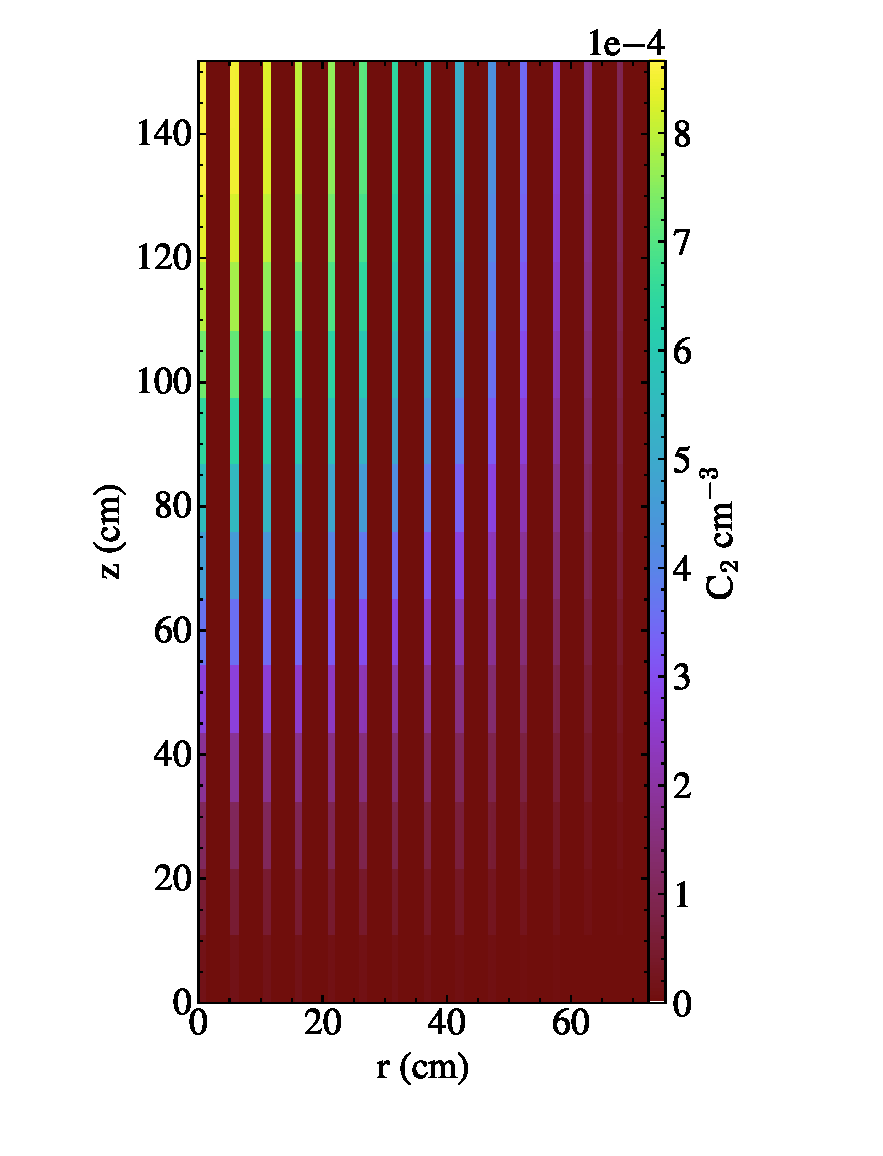
\includegraphics[width=0.28\textwidth]{./images/auto_diff_rho_pre2.eps}
   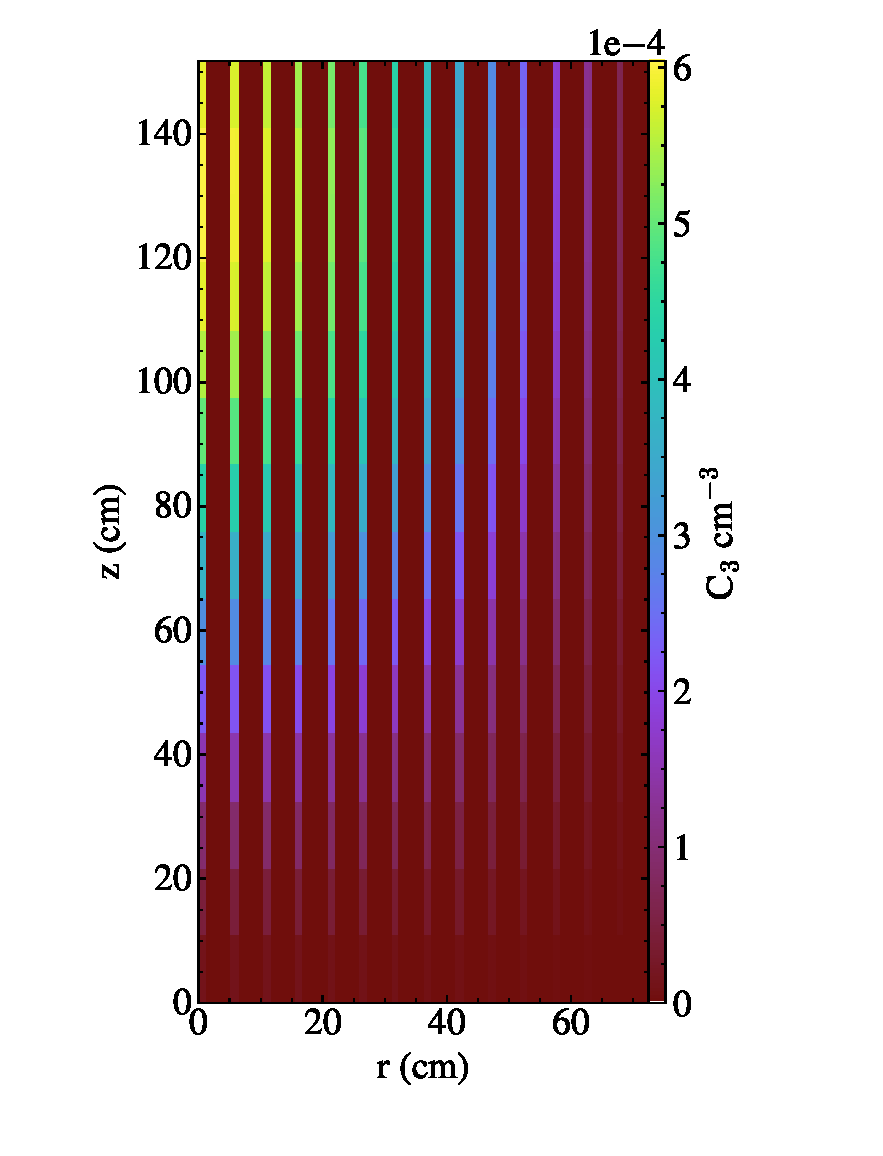
\includegraphics[width=0.28\textwidth]{./images/auto_diff_rho_pre3.eps}
   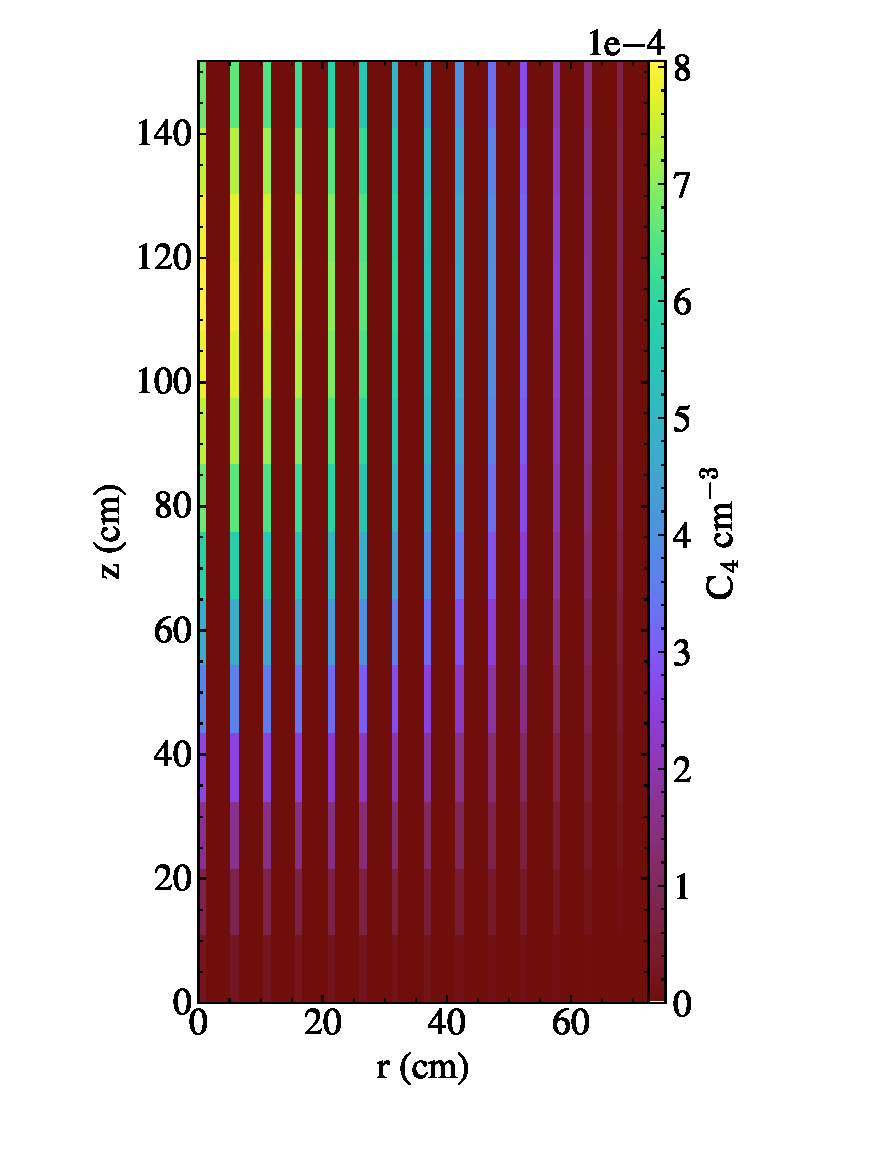
\includegraphics[width=0.28\textwidth]{./images/auto_diff_rho_pre4.eps}
   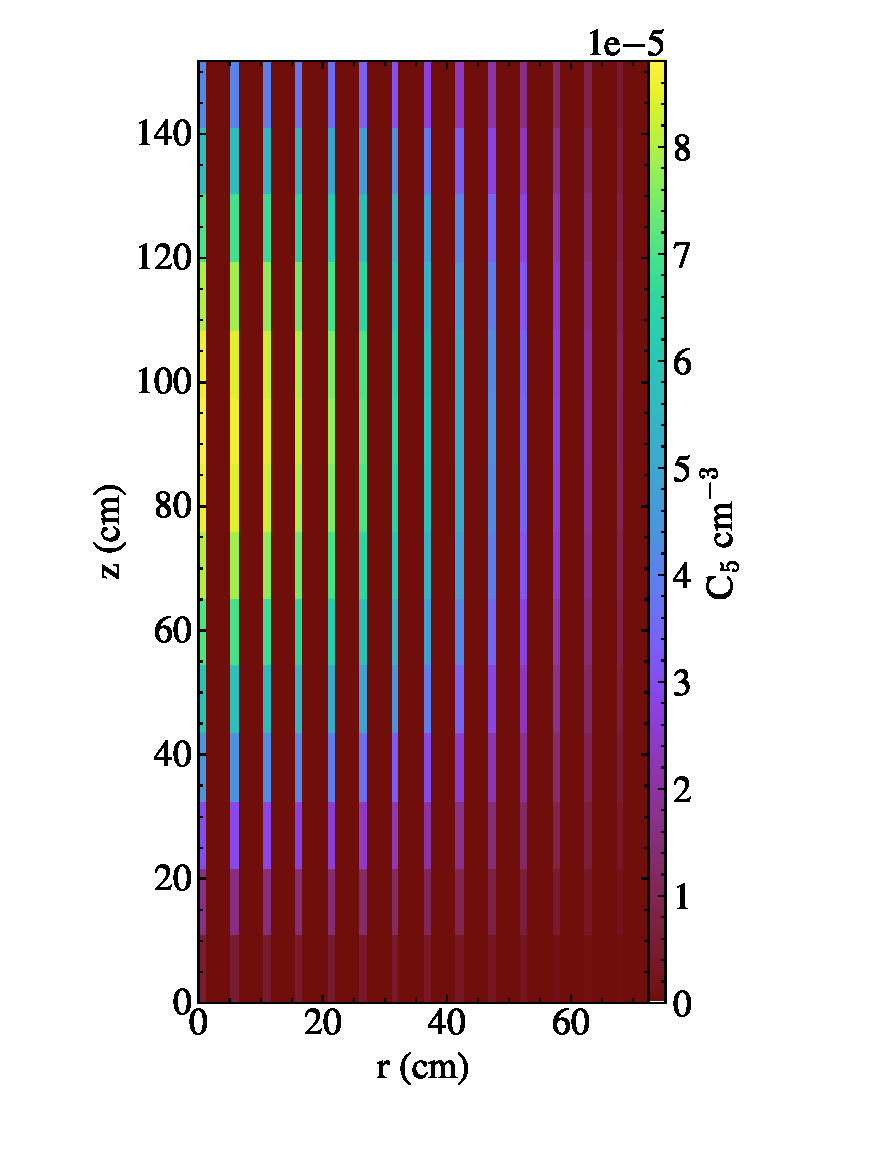
\includegraphics[width=0.28\textwidth]{./images/auto_diff_rho_pre5.eps}
   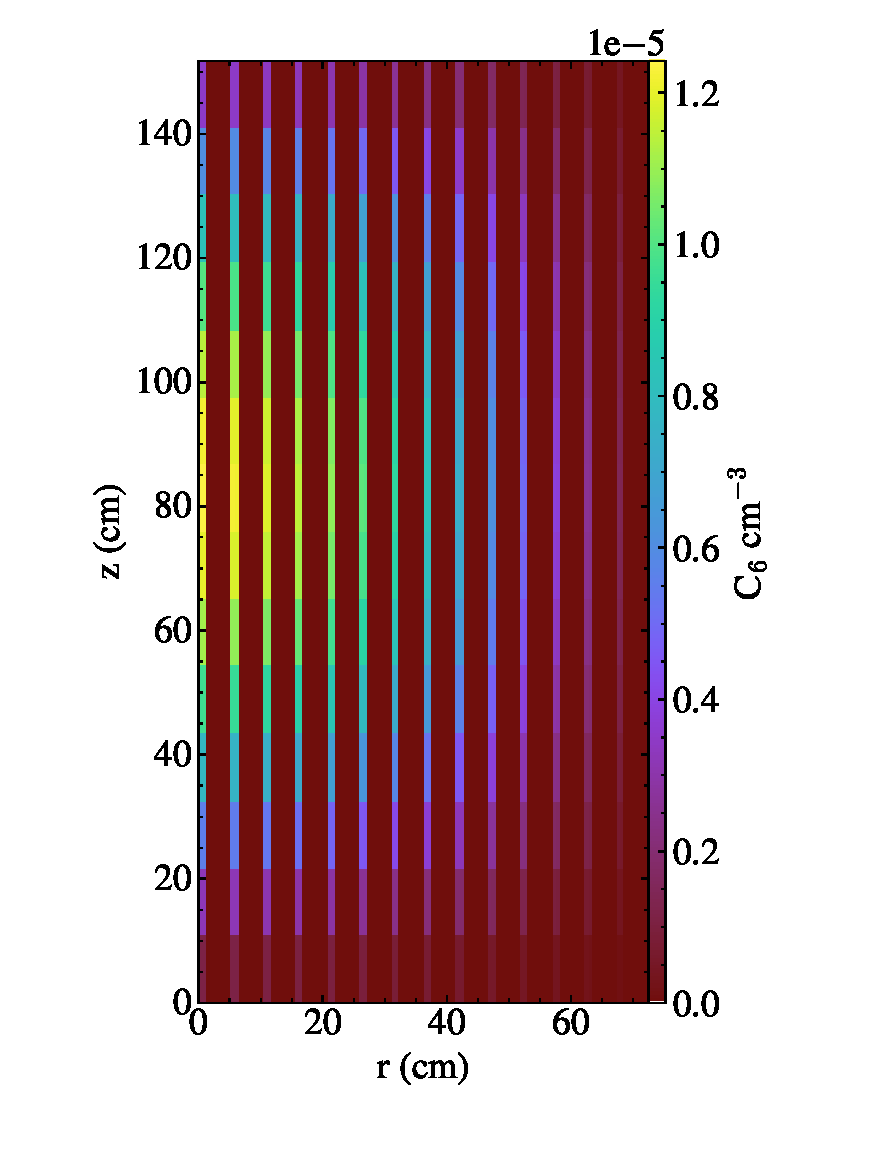
\includegraphics[width=0.28\textwidth]{./images/auto_diff_rho_pre6.eps}
    \end{figure}
\end{frame}



\begin{frame}
        \frametitle{Moltres MSRE Comparison}
  \begin{figure}
   \vspace{-0.05in}
   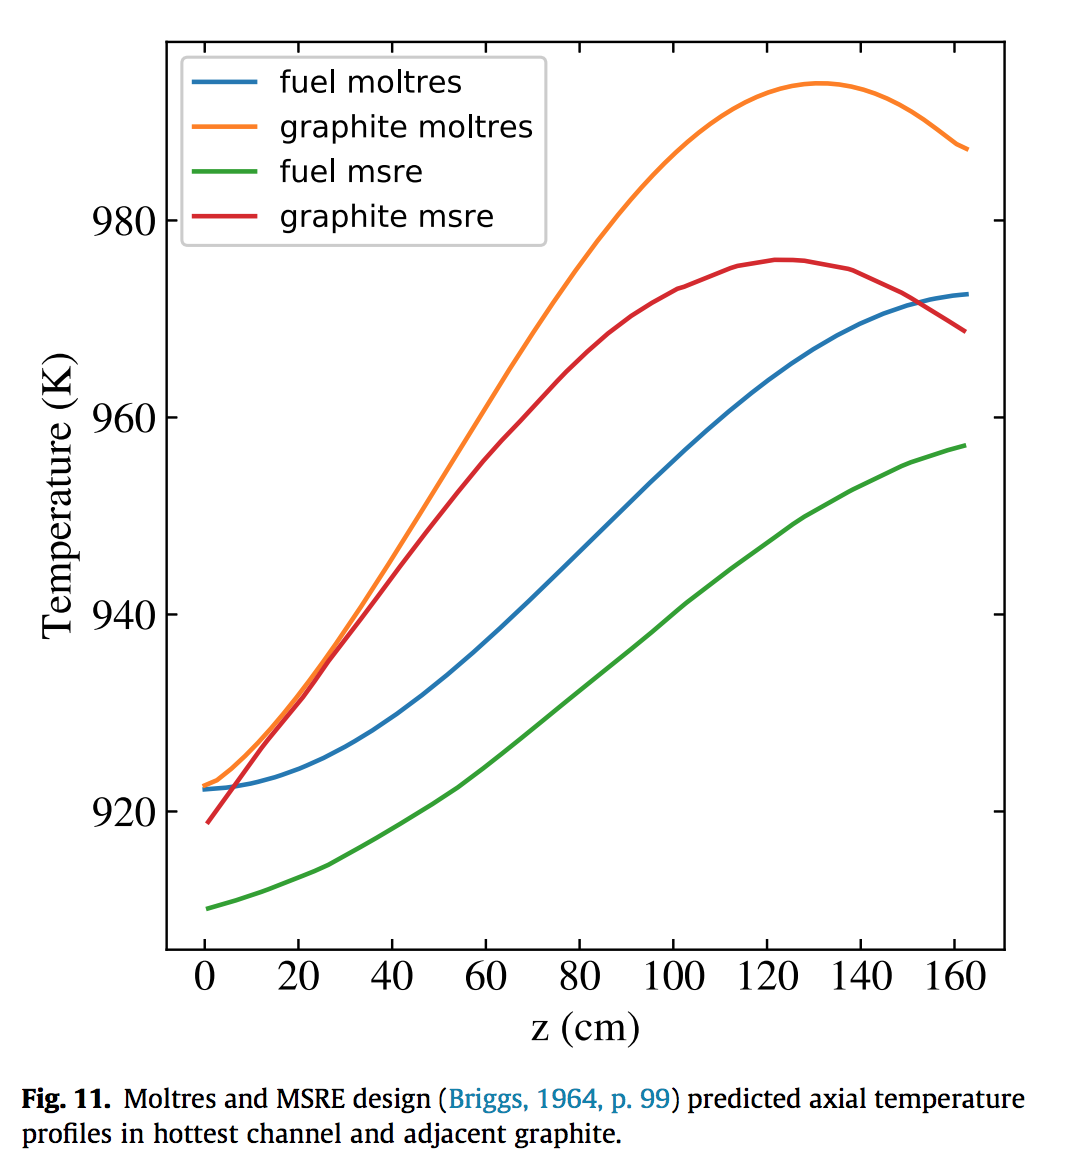
\includegraphics[height=0.85\textheight]{./images/moltres-axial.png}
    \end{figure}
\end{frame}


\begin{frame}
        \frametitle{Moltres MSRE Comparison}
  \begin{figure}
   \vspace{-0.05in}
   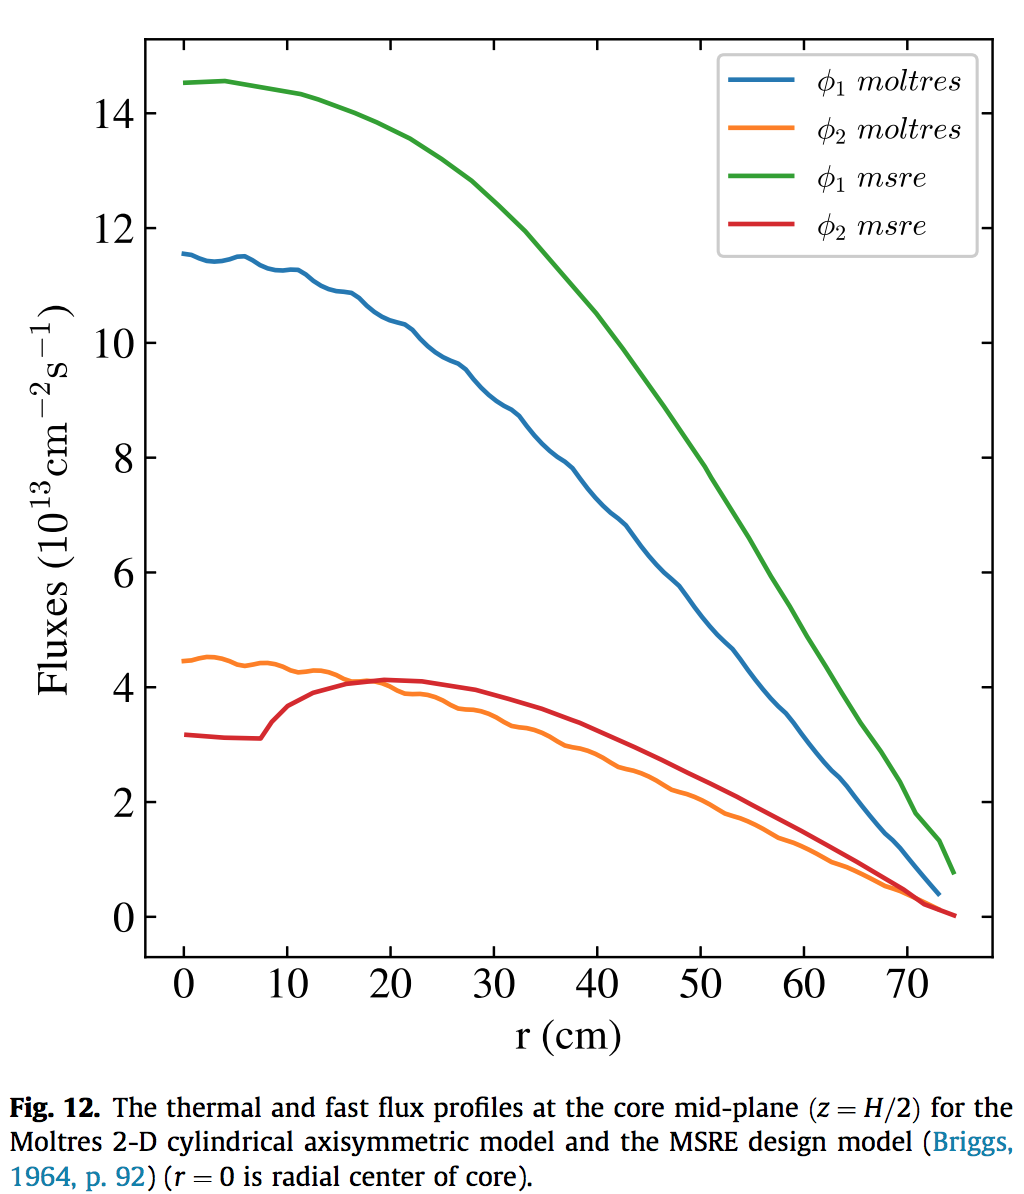
\includegraphics[height=0.85\textheight]{./images/moltres-axisym-flux.png}
    \end{figure}
\end{frame}


\begin{frame}
        \frametitle{Moltres MSRE Comparison}
  \begin{figure}
   \vspace{-0.05in}
   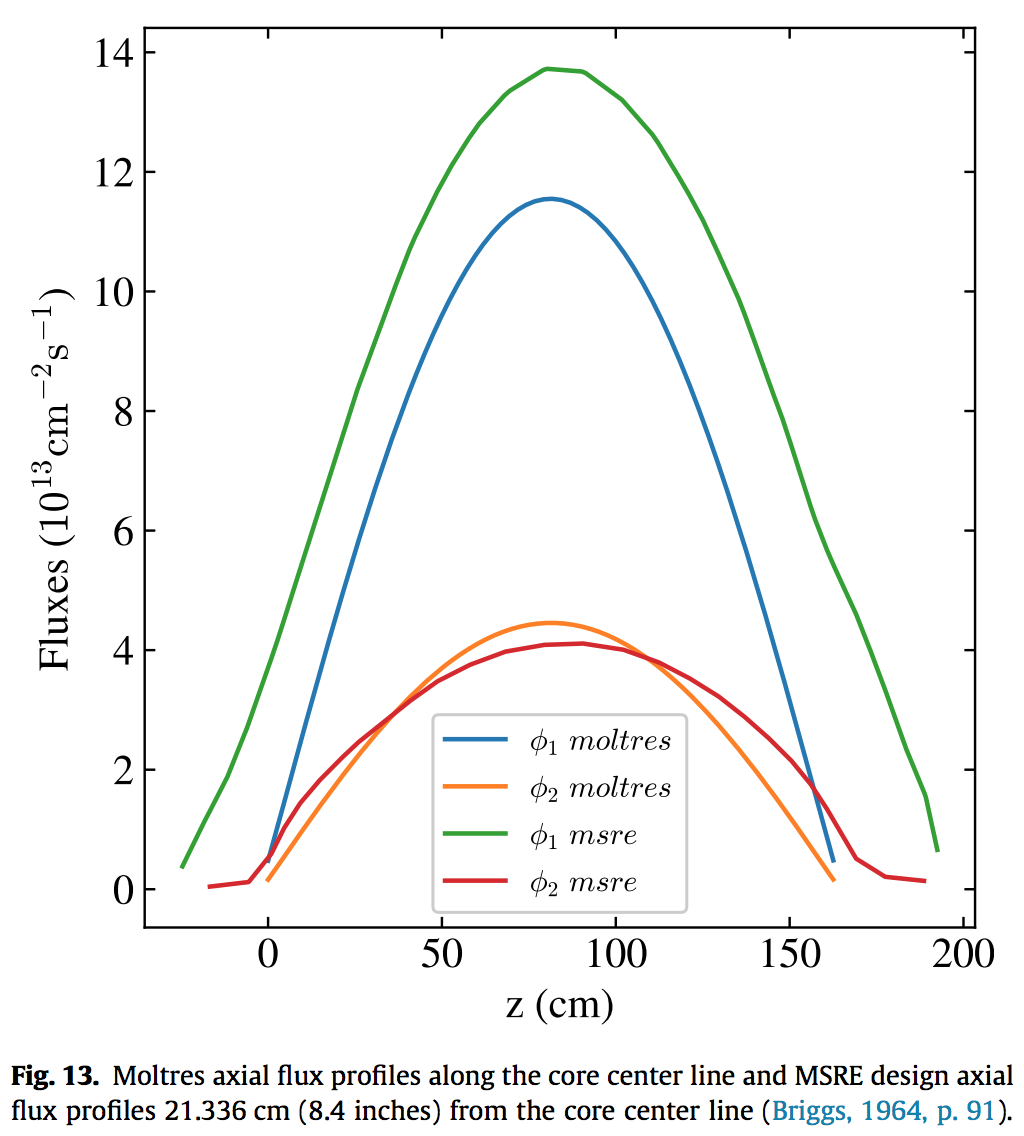
\includegraphics[height=0.85\textheight]{./images/moltres-axial-flux.png}
    \end{figure}
\end{frame}


\begin{frame}
  \frametitle{Multiphysics simulation results (3D)}
  \begin{figure}[t]
   \vspace{-0.1in}
   \hspace*{-0.45in}
   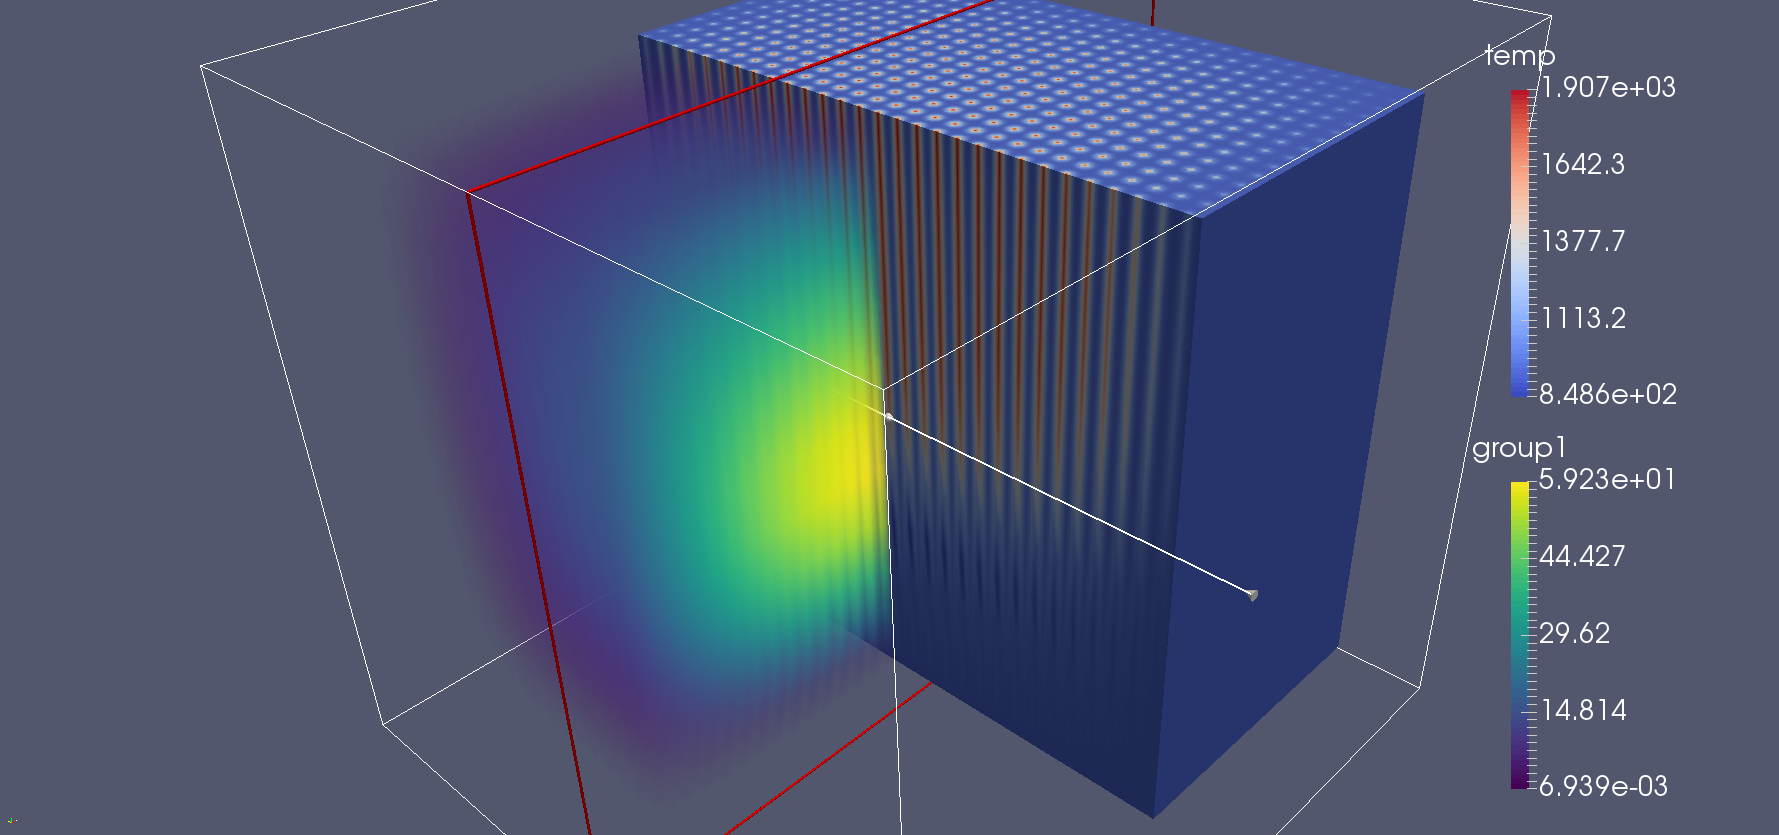
\includegraphics[height=0.75\textheight]{./images/moltres_3D.png}
   \caption{Cuboidal \gls{MSR} steady-state temperature and fast neutron flux 
          tests by Gavin Ridley.} 
    \end{figure}

\end{frame}
